%preambula
\documentclass[11pt]{article}

%packages
\usepackage[a4paper,
            total={17cm, 24cm},
            left=2cm,
            top=3cm,]{geometry}
\usepackage{babel}[czech]
\usepackage{times}
\usepackage{picture}
\usepackage[hidelinks]{hyperref}
\usepackage{multirow}
\usepackage[ruled,vlined]{algorithm2e}
\usepackage[utf8]{inputenc}
\usepackage[T1]{fontenc}
\usepackage{graphics}
\usepackage{amsmath}
\usepackage{graphicx}
\usepackage{pdflscape}
\usepackage{tikz}


%document
\begin{document}

    %titulna strana
    \begin{titlepage}
        \begin{center}
            \Huge\textsc{Vysoké učení technické v Brně}\\
            \huge\textsc{Fakulta informačních technologií}\\
            \vspace{\stretch{0.382}}
            {Typografie a publikování –– 3. projekt}\\
            \Huge{Tabulky a obrázky}\\
            \vspace{\stretch{0.618}}
        \end{center}
        {\LARGE 27. března 2024 \hfill
        Katarína Mečiarová (xmeciak00)}

    \end{titlepage}

%torzo
    \section{Úvodní strana}
    Název práce umístěte do zlatého řezu a nezapomeňte uvést dnešní datum a vaše jméno a příjmení.

    \section{Tabulky}
    Pro sázení tabulek můžeme použít bud prostředí \verb|tabbing| nebo prostředí \verb|tabular|.

    \subsection{Prostředí \texttt{tabbing}}
    Při použití \verb|tabbing| vypadá tabulka následovně:
    \begin{tabbing}
        Vodní melounyaa             \=aaaaaaaa              \=AAAAAAAAAA        \kill
        \textbf{Ovoce}      \> \textbf{Cena}        \> \textbf{Množství}        \\
        Jablka              \> 25,90                \> 3 kg                     \\
        Hrušky              \> 27,40                \> 2,5 kg                   \\
        Vodní melouny       \> 35,-                 \> 1 kus                    \\
    \end{tabbing}

    Toto prostředí se dá také použít pro sázení algoritmů, ovšem vhodnější je použít prostředí \verb|algorithm| nebo \verb|algorithm2e| (viz sekce 3).

    \subsection{Prostředí \texttt{tabular}}
    Další možností, jak vytvořit tabulku, je použít prostředí \verb|tabular|. Tabulky pak budou vypadat takto \footnote[1]{Kdyby byl problem s \texttt{cline}, zkuste se podívat třeba sem: \href{http://www.abclinuxu.cz/tex/poradna/show/325037}{http://www.abclinuxu.cz/tex/poradna/show/325037}.}:

    \begin{center}
        \begin{tabular}{|l|c|c|}
            \hline
            \multirow{2}{*}{\textbf{Měna}} &    \multicolumn{2}{|c|}{\textbf{Cena}} \\

                                                \cline { 2 - 3 }
                                                & \textbf{nákup}     & \textbf{prodej} \\

            \hline
            EUR         & 25,475    & 27,045    \\
            GBP         & 28,835    & 30,705    \\
            USD         & 22,943    & 24,357    \\
            \hline
        \end{tabular}
    \end{center}
    \begin{center}
        Tabulka 1: Tabulka kurzů $\mathrm{k}$ dnešnímu dni
    \end{center}

    \begin{center}
        \begin{tabular}{|c|c|}
            \hline
            A & $\neg A$ \\
            \hline
            \textbf{P} & N \\
            \hline
            \textbf{O} & O \\
            \hline
            \textbf{X} & X \\
            \hline
            \textbf{N} & P \\
            \hline
        \end{tabular}
        \begin{tabular}{|c|c|c|c|c|c|}
            \hline
            \multicolumn{2}{|c|}{\multirow{2}{*}{$A \wedge B$}} & \multicolumn{4}{|c|}{$B$} \\
            \cline{3-6}
            & & \textbf{P} & \textbf{O} & \textbf{X} & \textbf{N} \\
            \hline
            \multirow{4}{*}{A} & \textbf{P} & P & O & X & N \\
            \cline{2-6}
            & \textbf{O} & P & O & X & N \\
            \cline{2-6}
            & \textbf{X} & P & O & X & N \\
            \cline{2-6}
            & \textbf{N} & P & O & X & N \\
            \hline
        \end{tabular}
        \begin{tabular}{|c|c|c|c|c|c|}
            \hline
            \multicolumn{2}{|c|}{\multirow{2}{*}{$A \vee B$}} & \multicolumn{4}{|c|}{$B$}\\
            \cline{3-6}
            & & \textbf{P} & \textbf{O} & \textbf{X} & \textbf{N} \\
            \hline
            \multirow{4}{*}{A} & \textbf{P} & P & O & X & N \\
            \cline{2-6}
            & \textbf{O} & P & O & X & N \\
            \cline{2-6}
            & \textbf{X} & P & O & X & N \\
            \cline{2-6}
            & \textbf{N} & P & O & X & N \\
            \hline
        \end{tabular}
        \begin{tabular}{|c|c|c|c|c|c|}
            \hline
            \multicolumn{2}{|c|}{\multirow{2}{*}{$A \rightarrow B$}} & \multicolumn{4}{|c|}{$B$}\\
            \cline{3-6}
            & & \textbf{P} & \textbf{O} & \textbf{X} & \textbf{N} \\
            \hline
            \multirow{4}{*}{A} & \textbf{P} & P & O & X & N \\
            \cline{2-6}
            & \textbf{O} & P & O & X & N \\
            \cline{2-6}
            & \textbf{X} & P & O & X & N \\
            \cline{2-6}
            & \textbf{N} & P & O & X & N \\
            \hline
        \end{tabular}
    \end{center}



    \noindent{Tabulka 2: Protože Kleeneho trojhodnotová logika už je „zastaralá“, uvádíme si zde příklad čtyřhodnotové
    logiky}


    \section{Algoritmy}
    Pokud budeme chtít vysázet algoritmus, můžeme použít prostředí \verb|algorithm|\footnote[2]{Pro nápovědu,
        jak zacházet s prostředím \texttt{algorithm}, mužeme zkusit tuhle stránku: \href{http://ftp.cstug.cz/pub/tex/CTAN/macros/latex/contrib/algorithms/algorithms.pdf}{http://ftp.cstug.cz/pub/tex/CTAN/macros/latex/contrib/algorithms/algorithms.pdf}.} nebo \verb|algorithm2|\footnote[3]{Pro \texttt{algorithm2} zase tuhle: \href{http://ftp.cstug.cz/pub/tex/CTAN/macros/latex/contrib/algorithm2e/doc/algorithm2e.pdf}{http://ftp.cstug.cz/pub/tex/CTAN/macros/latex/contrib/algorithm2e/doc/algorithm2e.pdf}.}.
    Příklad použití prostředí \verb|algorithm2e| viz Algoritmus 1.

    \begin{algorithm}[H]
        \caption{FASTSLAM}
        \KwIn{$(X_{t-1}, u_t, z_t)$}
        \KwOut{$X_t$}
        \BlankLine
        $X_t^1 \leftarrow X_t = X_t' = 0$\;
        \For{$k=1$ to $M$}{
            $x_t^{[k]} \leftarrow$ sample\_motion\_model$(u_t, x_{t-1}^{[k]})$\;
            $\omega_t^{[k]} \leftarrow$ measurement\_model$(z_t, x_t^{[k]}, m_{t-1})$\;
            $m_t^{[k]} \leftarrow$ updated\_occupancy\_grid$(z_t, x_t^{[k]}, m_{t-1}^{[k]})$\;
            $X_t \leftarrow X_t + \langle x_t^{[k]}, \omega_t^{[k]} \rangle$\;
        }
        \For{$k=1$ to $M$}{
            draw $i$ with probability $\approx \omega_t^{[i]}$\;
            add $\langle x_t^{[k]}, m_t^{[k]} \rangle$ to $X_t$\;
        }
        \Return{$X_t$}\;
    \end{algorithm}

    \section{Obrázky}

    Do našich článků můžeme samozřejmě vkládat obrázky. Pokud je obrázkem fotografie, můžeme klidně použít bitmapový
    soubor. Pokud by to ale mělo být nějaké schéma nebo něco podobného, je dobrým zvykem takovýto obrázek vytvořit
    vektorově.\\

    \begin{center}
        \scalebox{0.35}{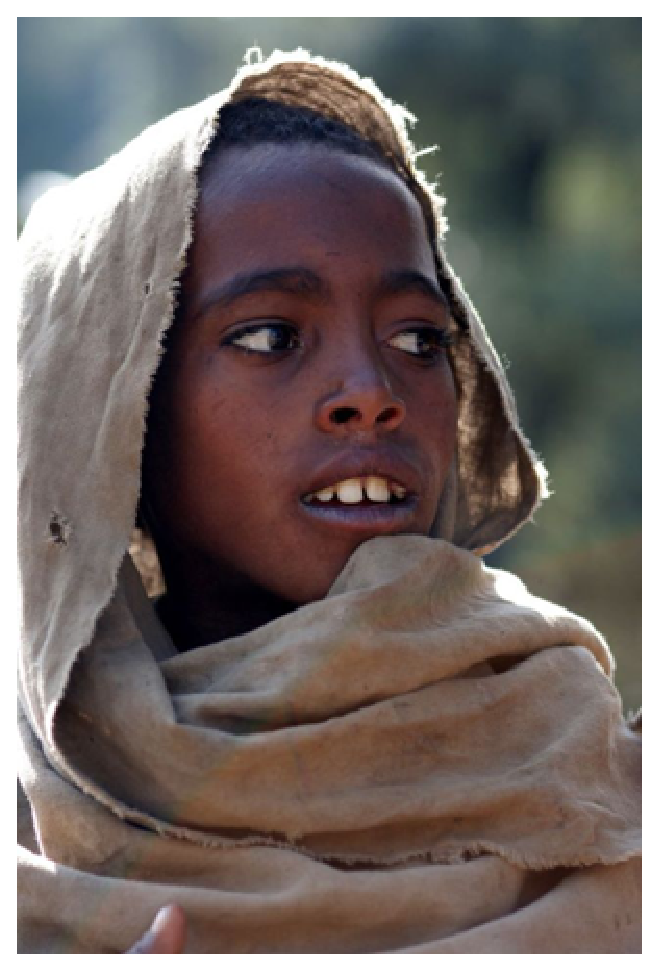
\includegraphics{etiopan} \reflectbox{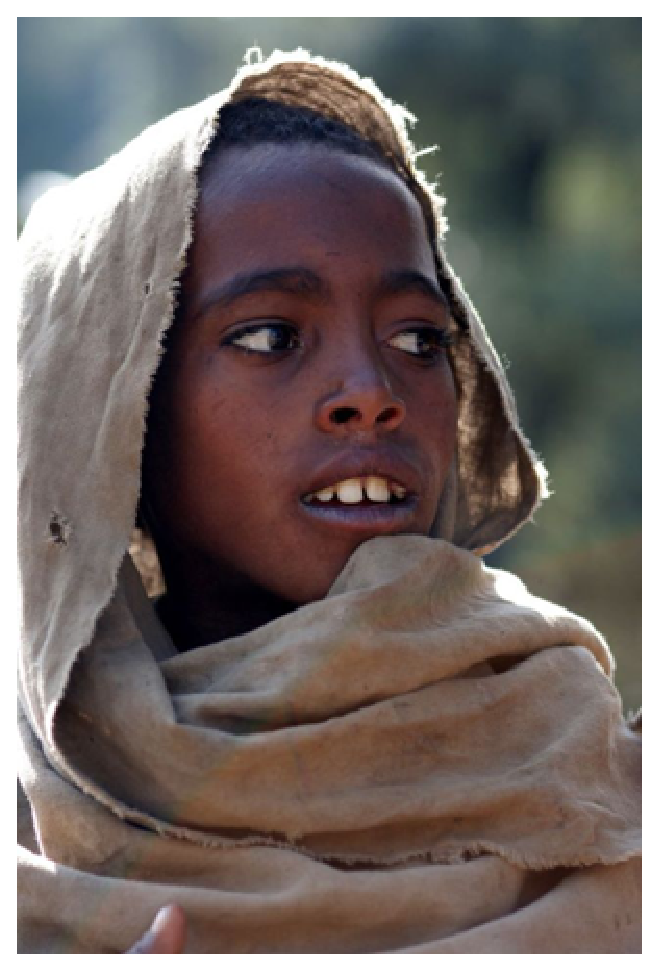
\includegraphics{etiopan}}}
    \end{center}

    \begin{center}
        Obrázek 1: Malý Etiopánek a jeho bratříček
    \end{center}
    \noindent{Rozdíl mezi vektorovým \ldots}

    \begin{center}
        \scalebox{0.35}{
\includegraphics{oniisan}}
    \end{center}

    \begin{center}
        Obrázek 2: Vektorový obrázek
    \end{center}


    \noindent{\ldots a bitmapovým obrázkem}

    \begin{center}
        \scalebox{0.6}{
\includegraphics{oniisan2.eps}}
    \end{center}

    \begin{center}
        Obrázek 3: Bitmapový obrázek
    \end{center}


    \noindent{se projeví například při zvětšení.}

    Odkazy (nejen ty) na obrázky 1,2 a 3, na tabulky 1 a 2 a také na algoritmus 1 jsou udělány pomocí křížových odkazů.
    Pak je ovšem potřeba zdrojový soubor přeložit dvakrát.
    Vektorové obrázky lze vytvořit i přímo v \LaTeX u, například pomocí prostředí \verb|picture|.

    \newpage
    \begin{landscape}
    %TODO your own home
        \begin{figure}[h]
            \centering
            \setlength{\unitlength}{1mm}
            \begin{picture}(180,120) % A5 landscape size
                % Frame
                \put(0,0){\framebox(180,120){}}
                % House
                \put(20,20){\includegraphics[width=40mm]{example-image-a}} % Replace example-image-a with your house image
                % Roof
                \put(20,60){\line(1,2){10}}
                \put(60,60){\line(-1,2){10}}
                \put(20,60){\line(1,0){40}}
                % Chimney
                \put(30,85){\line(1,0){10}}
                \put(30,85){\line(0,1){8}}
                \put(40,85){\line(0,1){8}}
                \put(30,93){\line(1,0){10}}
                % Door
                \put(30,20){\line(0,1){30}}
                \put(30,25){\circle*{2}}
                % Windows
                \put(25,30){\line(1,0){10}}
                \put(25,30){\line(0,1){10}}
                \put(35,30){\line(0,1){10}}
                \put(25,40){\line(1,0){10}}
                \put(55,30){\line(1,0){10}}
                \put(55,30){\line(0,1){10}}
                \put(55,40){\line(1,0){10}}
                \put(65,30){\line(0,1){10}}
                % Flowerbed
                \put(50,20){\line(1,0){20}}
                \put(50,20){\line(0,1){5}}
                \put(70,20){\line(0,1){5}}
                \put(50,25){\line(1,0){20}}
                \put(55,25){\circle*{2}}
                \put(65,25){\circle*{2}}
                % Path
                \put(15,20){\line(0,1){2}}
                \put(15,20){\line(1,0){5}}
                \put(20,20){\line(0,1){5}}
            \end{picture}
            \label{fig:modern_house}
        \end{figure}

    \noindent{Obrázek 4: Vektorový obrázek moderního bydlení vhodného pro 21. století. (Bud to vytvořte stejný obrázek, anebo nakreslete pomocí picture váš vlastní domov.)}

    \end{landscape}

\end{document}